\documentclass{article}   	                         % use "amsart" instead of "article" for AMSLaTeX format
\usepackage{geometry}                		% See geometry.pdf to learn the layout options. There are lots.
\geometry{letterpaper}                   		% ... or a4paper or a5paper or ... 
%\geometry{landscape}                		% Activate for rotated page geometry
%\usepackage[parfill]{parskip}    		% Activate to begin paragraphs with an empty line rather than an indent
\usepackage{graphicx}				% Use pdf, png, jpg, or eps§ with pdflatex; use eps in DVI mode
\graphicspath{ {./images/} }								% TeX will automatically convert eps --> pdf in pdflatex		
\usepackage{amssymb}

%SetFonts

%SetFonts


\title{Game Theory And Its Applications}
\author{Sambit Behera}
\date{April-May 2020}							% Activate to display a given date or no date
\begin{document}

\maketitle

\tableofcontents

\section{Preface}

%\subsection{}

Welcome to my Summer Of Science report on Game Theory And Its Applications. This is an attempt to summarise all the sub-topics I cover in this journey. I would mostly follow the book \textbf{An Introduction To Game Theory} by \textbf{Levent Koçkesen} and \textbf{Efe A. Ok}. Also, I would be referring to Game Theory course on Coursera for additional knowledge. I hope this report would be helpful to gain a decent understanding of Game Theory.

\begin{flushleft}
\section{Introduction}
\end{flushleft}
\subsection{Game Theory}
In a game as simple as Rock, Paper, Scissors, when two people play their respective moves at a time, they hope to play the move that is in favour of them and eventually win the game. The strategy applied by both the users, like looking for a pattern in their opponents' previous moves to predict their next move, is what makes up a part of this topic. Largely popularised by the famous movie \textit{A Beautiful Mind}, based on the life of Nobel winning laureate \textbf{John Nash}, Game Theory is essentially the science of strategy, or at least the optimal decision-making of independent and competing actors in a strategic setting.
\subsection{Basic Terminologies}
	\begin{itemize}
	\item \textbf{Players:}\\
	The strategic decison-makers in the context of the game. These can be as small as individuals and as large as governments or multi-national companies.
	\item \textbf{Rational:}\\
		An individual is considered \textit{rational} if she has well defined objectives (or preferences) over the set of possible outcomes and she implements the best available \textit{strategy} to pursue them. In reality, assumption of rationality might be an unrealistic one. These limitations is what gives birth to the concept of \textit{bounded rationality} which is an active area of research currently.
	\item \textbf{Strategy:}\\
	A proper set of action plans chosen by a player in a certain setting, whose outcome depends not only on her action, but on others' too.
	\item \textbf{Rules:}\\
	A set of statements that clarifies, demarcates and/or interprets the proceedings of a game.  
	\item \textbf{Actions:}\\
	These are the choices available to the player from which she has to choose.
	\item \textbf{Payoff:}\\
	Sounds like a reward, it acts as a motivating factor behind the actions of the players and the reason for their participation.
	\item \textbf{Common Knowledge:}\\
	As we consider all players in the game to be \textit{rational}, everyone of the players knows about the model, everybody knows that everybody knows about the model, everybody knows that everybody knows that everybody knows it, and so on.
	\end{itemize}
\pagebreak
`\section{Dominant Strategies and Equilibrium}

In certain situations,  a player may have strategic options to choose for his best move, and each move would have its corresponding payoff. As the player is considered $rational$, he would prefer the move with the best possible payoff. Hence, this move is said to $dominate$ over the others. There are various forms of dominance.

\subsection{Strongly Dominant Strategy}
Let $s_i$ and $s'_i$ be two strategies for player $i$, and let $S_{-i}$ be the set of all possible strategy profile for the other players, then $s_i$ is said to $strongly$ $dominate$ over $s'_i$ if, $$u_i(s_i, s_{-i})> u_i(s'_i, s_{-i}) \forall s_{-i} \in S_{-i}$$
Hence, it is obvious that player $i$ will always prefer strategy $s_i$ over $s'_i$.

\subsection{Very Weakly Dominant Strategy}

We say that strategy $s_i$ is \textit{weakly dominant} over $s'_i$ if, $$u_i(s_i, s_{-i}) \geq u_i(s'_i, s_{-i}) \forall s_{-i} \in S_{-i}$$
Here, the dominance is not strict.\\
There also are other kinds of dominant strategies that lie between the above two extremes., which we would talk about later in the report.
\subsection{Dominance and Equilibrium}

\subsubsection{Strongly Dominant Strategy Equilibrium}

A strategy profile $(s^*_1, \dots , s^*_n)$ is called a \textit{strongly dominant strategy equilibrium} of a game, if $\forall i = 1, 2, \dots , n$ the strategy $s^*_i$ is a strongly dominant strategy for player $i$. 

\subsubsection{Very Weakly Dominant Strategy Equilibrium}

A strategy profile $(s^*_1, \dots , s^*_n)$ is called a \textit{very weakly dominant strategy equilibrium} of a game, if $\forall i = 1, 2, \dots , n$ the strategy $s^*_i$ is a very weakly dominant strategy for player $i$. 


\pagebreak
\section {Nash Equilibrium}

\subsection{Definition}
It is a stable state of a game involving the interaction of different participants, in which no participant can gain by a unilateral change of strategy if the strategies of the others remain unchanged. \\

\begin{flushleft}\textit{Nash Equilibrium} of a game $G$ in strategic form is defined as any outcome $(a^*_1, \dots , a^*_n)$ such that \end{flushleft}$$u_i(a^*_i, a^*_{-i}) \geq u_i(a_i, a^*_{-i})\hspace{0.3cm} \forall a_i \in A_i$$ holds for each player $i$. The set of all Nash equilibria of $G$ is denoted by $N(G)$.

\subsection{Best Response}
We define the \textit{Best Response correspondence}\footnote{By definition, a \textit{correspondence} $f$ from $A$ to $B$ assigns to each $x \in A$ a \textit{subset} of $B$, and hence we write $f: A \rightrightarrows B$} of a player $i$ in a strategic form game as the correspondence$B_i : A_{-i} \rightrightarrows A_i$ given by $$B_i(a_{-i}) = \{a_i \in a_i: u_i(a_i, a_{-i}) \geq u_i(b_i, a_{-i})\hspace{0.2cm} \forall b_i \in A_i\} $$

\subsection{Pure Strategy Nash Equilibrium}
Given a normal form game $\mathcal{T} = \langle \mathcal{N}, (A_i)_{i \in N}, (u_i)_{i \in N}\rangle$, the action profile $A^* = (a^*_1, \dots , a^*_n)$ is called a \textit{pure strategy Nash Equilibrium of $\mathcal{T}$ if} $\forall i, a^*_i$ belongs to the set of \textit{best response } of $a^*_{-i}$.

\begin{flushleft}In words, we can say that this Nash Equilibrium strategy is the best response to the Nash Equilibrium strategies of the other players. \newline

\begin{large}\textbf{Application on Some Example Games}\end{large}\end{flushleft}

\begin{flushleft}\textbf{Prisoners' Dilemma}\end{flushleft}
Consider the following story:\\
Two suspects are arrested and put into different cells before the trial. The district attorney, who is pretty sure that both of the suspects are guilty but lacks enough evidence, offers them the following deal: If both of them confess and implicate the other (labeled $C$), then each will be sentenced to, say, 3 years of prison time. If one confesses and the other does not (labeled $N$), then the “rat” goes free for his cooperation with the authorities and the non-confessor is sentenced to 4 years of prison time. Finally, if neither of them confesses, then both suspects get to serve 1 year. 

Now, Let's analyse this case. The corresponding matrix will be- 
\begin{center}\begin{tabular}{|c|c|c|} \hline
1/2 & $C$ & $N$ \\ \hline
$C$ & -3,-3 & 0,-4 \\ \hline
$N$ & -4,0 & -1,-1 \\ \hline 
\end{tabular}\end{center}

\begin{itemize}
\item First consider that the suspect 2 chooses to confess and implicate the other $ie$ chooses $C$. Then, the best response for suspect 1 would be to confess rather than not, as it has lesser prison time. 
\item If we consider suspect 2 to not confess, then suspect 1 has the option to "rat" out 1 and walk free. We can consider similar cases for suspect 2.
\end{itemize}
We see that no matter what the other suspect does, it is in the best interest of each suspect to rat out the other as this is the best response in any situation. Hence, we can say that choosing $C$ is the \textit{strongly dominant strategy}. Hence, we can conclude that $CC$ is the \textit{pure strategy Nash Equilibrium} here.\newline

Let's consider the \textbf{Coordination Game} described in \textbf{section 2.4}. Here's the matrix for it-

		\begin{center}
		\begin{tabular}{|c|c|c|}\hline
		$1/2$ & Left & Right \\ \hline
		Left &  1,1 & -1,-1 \\ \hline
		Right & -1,-1 & 1,1 \\ \hline
		\end{tabular}
		\end{center}
We can see that we have \textit{two Nash equilibria} here. If one of the drivers goes to the left, it's the best response to go to the left. And conversely, if the the other driver goes to the right, then the first driver is best off going to the right as well. And the others are not Nash equilibria.

\subsection{Pareto Dominance and Optimality}

Till now, we have been considering the whole game scenario as a participant in it. But there should be a proper approach from the point of view of an outside observer who has no obligation to any of the players. The observer might prefer a certain outcome as kind of a social good of the participants.\newline

Sometimes one outcome $o$ is atleast as good for every agent as another outcome $o'$, and there is some agent who $strictly$ prefers $o$ to $o'$. In this case, it is reasonable to say that $o$ is better than $o'$. 
\begin{center}We say that $o$ \textit{Pareto-dominates} $o'$\end{center}

\begin{large}\textbf{Pareto optimality}\end{large}\newline\

An outcome $o^*$ is \textbf{Pareto-optimal} if there is no other outcome that \textit{Pareto-dominates} it.
\begin{flushleft}
\textbf{Proposition 1:} It is possible for a game to have more than one Pareto-optimal outcome.\newline

\textit{Proof:} A game might have exactly same payoff values that are also Pareto-dominant over others for different action combinations, hence none of them is Pareto-dominant over each other and both are Pareto-optimal.\newline

\textbf{Proposition 2:} Every game has atleast one Pareto-optimal outcome.\newline

\textit{Proof:} For some outcome to not be Pareto-optimal it has to be dominated by some other outcome. And if it is dominated by some outcome, then the dominant outcome would be considered for Pareto-optimality and so goes on the cycle. Hence, a game has to have a Pareto-optimal outcome.
\end{flushleft}

\textbf{Matching Pennies}\\

Let's consider a new example game called \textit{Matching Pennies}.  . It is played between two players, Even and Odd. Each player has a penny and must secretly turn the penny to heads or tails. The players then reveal their choices simultaneously. If the pennies match (both heads or both tails), then Even keeps both pennies and hence his payoff is $+1$ and it is $-1$ for Odd. But if the pennies do not match, then the payoff is $+1$ for Odd and $-1$ for Even.\newline
Here's the following matrix for it-
	         \begin{center}
		\begin{tabular}{|c|c|c|}\hline
		Even/Odd & Heads & Tails \\ \hline
		Heads &  1,-1 & -1,1 \\ \hline
		Tails & -1,1 & 1,-1 \\ \hline
		\end{tabular}
		\end{center}
Here, we can see that in search of best response, we are lead into a cycle. Hence, there is no pure strategy Nash Equilibrium.
Now, if we consider Pareto Dominance, no move dominates another move, hence \textit{by definition}, every strategy is a \textit{Pareto Optimal} strategy.

\pagebreak
\section{Mixed Strategies and Nash Equilibrium}

\subsection{Mixed Strategy}
\hspace{1cm}Consider a scenario, where there is a conflict between the Mafia and the Army. The Mafia wants to attack one of several trade routes randomly for loot, but would lose if the Army is guarding it. If the Army plays a fixed strategy to guard only certain routes (as we do in pure strategy equilibrium) then the Mafia will be able to understand the plan and attack the ones not being guarded at a particular time. Hence, the Army has to play mixed strategy to make it difficult for the Mafia to figure out a way to loot.\newline

Let's reconsider the \textit{Matching Pennies} game in the previous section. It would be a pretty bad idea to play any deterministic strategy in this game. So, a basic approach would be to confuse the opponent by playing randomly. In this way, there is no sure approach and hence we have a \textit{positive probability} for each action being played.\\

 So, we re-define a \textbf{strategy} $s_i$ for agent $i$ as any  probability distribution over the actions $A_i$-
 \begin{itemize}
 \item \textbf{pure strategy:} only one action is played with positive probability.
 \item \textbf{mixed strategy:} more than one action is being played with positive probability
 	\begin{itemize}
	\item These actions are called the \textbf{support} of the mixed strategy
	\end{itemize}
 \end{itemize}
 
 If the set of all \textit{strategies} for $i$ be $S_i$, then the set of \textit{all strategy profiles }will be $S = S_1 \times \dots \times S_n$\newline
 
\textbf{Payoff/Utility under Mixed strategies}\\

If all the players follow mixed strategy profile $s \in S$, the payoff won't be as simple as reading it from the game matrix. Instead, we would use the idea of \textit{expected utility} as follows:
	$$u_i(s) = \sum_{a \in A} u_i(a) Pr(a|s)$$
	where,$$Pr(a|s) = \prod_{j \in N}s_j(a_j)$$
	Here, $u_i(s)$ is the utility of a player $i$ who played the strategy profile $s$ and $Pr$ is the probability that we get to an action $a$ given we choose strategy profile $s$.

\subsection{Best Response and Nash Equilibrium}

Previously in \textbf{section 4}, we used actions to determine the best response and hence Nash Equilibrium. Now, we can generalise the definition to use strategies to determine the best response.\newline

\begin{flushleft}\textbf{Best Response}:\\ \begin{center} $s_i^*\in BR(s_{-i})$ $iff$ $\forall s_i \in S_i, u_i(s_i^*, s_{-i}) \geq u_i(s_i, s_{-i})$\end{center}
Hence, there we can be multiple best responses.\newline

\textbf{Nash Equilibrium}
$$s = \langle s_1, \dots , s_n\rangle \textit{ is a Nash Equilibrium iff } \forall i, s \in BR{s_{-i}}$$
\end{flushleft}

If we reconsider the \textit{Matching Pennies} game, we had no pure strategy Nash Equilibrium. But, if consider a probabilistic approach to the choice of Head or Tail, \textit{ie} a $0.5$ probability for both, then we have a mixed strategy Nash Equilibrium.

\subsection{Computing Mixed Nash Equilibrium}
A mixed strategy profile is a Nash Equilibrium if and only if the utility of the profile is same for both players and is greater than all other possible utilities for different actions.\newline
\begin{flushleft}Let's consider the \textit{Battle Of The Sexes} game in section 2.4. 
\end{flushleft}
	\begin{center}
	\begin{tabular}{|c|c|c|}\hline
	Husband/Wife & Movie A & Movie B \\ \hline
	Movie A &  2,1 & 0,0 \\ \hline
	Movie B & 0,0 & 1,2 \\ \hline
	\end{tabular}
	\end{center}
	
	Nash equilibrium is achieved if one player sets his probability such that the options for other player become indifferent, \textit{ie} any of the actions will give equal payoff to the second player. We can ensure that by solving a linear equation to find the corresponding probability. 

Assume the Wife opts for Movie A with probability $p$ and B with probability $1-p$. Then,
\begin{eqnarray}
u_1(A, s^*_2) &=& 2 (p) + 0(1-p) = 2p\\
u_1(B, s^*_2) &=& 0 (p) + 1(1-p)= 1-p\\
u_1(B, s^*_2) &=& u_1(A, s^*_2) \\
p &=& \frac{1}{3}
\end{eqnarray}	
Similarly, to make the options for wife indifferent, we have to find the probability $q$ with which Husband chooses the movie A
\begin{eqnarray}
u_2(A, s^*_1) &=& 1 (q) + 0(1-q) = 1q\\
u_2(B, s^*_1) &=& 0 (q) + 2(1-q)= 2 - 2q\\
u_2(B, s^*_1) &=& u_2(A, s^*_1) \\
q &=& \frac{2}{3}
\end{eqnarray}	

Hence, the strategy profile$ \left( \left(\displaystyle{\frac{2}{3}},\displaystyle{\frac{2}{3}}\right),\left(\displaystyle{\frac{2}{3}},\displaystyle{\frac{2}{3}}\right)\right)$ results in Nash Equilibrium.
\subsection{Theorem - Nash, 1950}
$$\textit{Every finite game has a Nash Equilibrium}$$

\pagebreak
\section{Alternate Solution Concepts}

\subsection{Strictly Dominated Strategies}
This is a type of strategy which is never a best reply. Essentially, this is a startegy we can safely ignore.

In terms of formal notation, A strategy $a_i \in A_i$ is strictly dominated by $a_i^* \in A_i$ if $$u_i(a_i, a_{-i}) < u_i(a_i^*, a_{-i}) \hspace{0.2cm} \forall a_{-i} \in A_{-i}$$

\subsection{Iterated Removal Of Strictly Dominated Strategies}

If in a game, we come across a strictly dominated strategy, we can reduce the possibility of playing that strategy to $0$. Essentially, we remove that strategy altogether. By applying such removal startegy, we can collapse the game to a much simpler one for us to analyze and apply the solution concepts.\\

Let's consider a 3-by-3 normal form game given below:\\
		\begin{center}
		\begin{tabular}{|c|c|c|c|}\hline
		$1/2$ & Left & Middle & Right\\ \hline
		Top &  3,0 & 2,1 & 0,0 \\ \hline
		Middle & 1,1 & 1,1 & 5,0 \\ \hline
		Bottom & 0,1 & 4,2 & 0,1 \\ \hline
		\end{tabular}
		\end{center}
		
We can easily see that payoff for Player 2 is always less while playing Right strategy than the other two strategies. This points out that this strategy is \textit{strictly dominated} by the others and we can easily remove the column from our matrix as follows.

		\begin{center}
		\begin{tabular}{|c|c|c|}\hline
		$1/2$ & Left & Middle \\ \hline
		Top &  3,0 & 2,1  \\ \hline
		Middle & 1,1 & 1,1 \\ \hline
		Bottom & 0,1 & 4,2 \\ \hline
		\end{tabular}
		\end{center}
		
Now, we consider the Middle strategy for Player 1 and conclude that it is a  \textit{strictly dominated strategy} too and the matrix can be further simplified.

		\begin{center}
		\begin{tabular}{|c|c|c|}\hline
		$1/2$ & Left & Middle \\ \hline
		Top &  3,0 & 2,1   \\ \hline
		Bottom & 0,1 & 4,2 \\ \hline
		\end{tabular}
		\end{center}
		
Again, Left strategy for Player 1 is now  \textit{strictly dominated strategy} and can be removed. 
		\begin{center}
		\begin{tabular}{|c|c|c|}\hline
		$1/2$ & Middle \\ \hline
		Top  & 2,1   \\ \hline
		Bottom & 4,2 \\ \hline
		\end{tabular}
		\end{center}

From the following \textit{Iterated Removal} we can conclude that the strategy profile \{Bottom, Middle\} is in Nash Equilibrium.

\begin{flushleft}\textbf{Few Points}\end{flushleft}
\begin{itemize}
\item This strategy preserves \textit{Nash Equilibrium}.
\item It can be used as a preprocessing step before computing an equilibrium.
\item Games that are solvable by this technique are called \textbf{Dominance Solvable} games .
\item Order of removal doesn't matter in case of multiple strictly dominated strategies .
\end{itemize}

\subsection{Weakly Dominated Strategies}
A strategy is \textit{weakly dominated} by $a_i^* \in A_i$ if $$u_i(a_i, a_{-i}) \leq u_i(a_i^*, a_{-i}) \hspace{0.2cm} \textit{for all }  a_{-i} \in A_{-i}$$ and $$u_i(a_i, a_{-i}) < u_i(a_i^*, a_{-i}) \hspace{0.2cm} \textit{for some } a_{-i} \in A_{-i}$$.

In this strategy, we can use iterated removal to remove the weakly dominated strategies but with precaution because:

\begin{itemize}
\item Such strategies can be best replies
\item Order of removal can matter
\item Atleast one equilibrium is preserved
\end{itemize}

\subsection{Maxmin Strategies}

Player $i$'s \textit{maxmin strategy} is a strategy that maximizes $i$'s worst-case payoff, in the situation where all the players happen to play the strategies which cause the greatest harm to $i$.\\

The \textit{maxmin value} of the game for player $i$ is the minimum payoff guaranteed by a maxmin strategy.\\
\begin{flushleft}
\textbf{Definition:}
\end{flushleft}
The \textbf{maxmin strategy} for player $i$ is $$arg \hspace{0.1cm}max_{s_i} min_{s_{-i}} u_i(s_1, s_2)$$ and the \textbf{maxmin value} for player is  $$max_{s_i} min_{s_{-i}} u_i(s_1, s_2)$$

\subsection{Minmax Strategies}

Player $i$'s \textit{minmax strategy} against player $-i$ in a 2-player game is a strategy that minimizes $-i$'s best-case payoff, and the \textit{minmax value} for $i$ against $-i$ is payoff.

\begin{flushleft}
\textbf{Definition:}
\end{flushleft}
In a 2-player game, the \textbf{minmax strategy} for player $i$ against player $-i$ is $$arg \hspace{0.1cm}min_{s_i} max_{s_{-i}} u_i(s_1, s_2)$$ and the \textbf{minmax value} for player $-i$ is  $$min_{s_i} max_{s_{-i}} u_i(s_1, s_2)$$

\subsection{Minmax Theorem - \textit{von Neumann}, 1928}
\textit{In any finite, two-player, zero sum game, in any Nash Equilibrium each player receives a payoff that is equal to both his maxmin and minmax value.}
\begin{enumerate}
\item Each player's maxmin value is equal to his minmax value.The maxmin value for player I is called the \textit{value of the game}
\item For both players, set of minmax strategies coincides with the set of maxmin strategies.
\item Any maxmin strategy profile (or, equivalently, minmax strategy profile) is a Nash Equilibrium. Furthermore, these are all the Nash equilibria. Consequently, all Nash equilibria have the same payoff vector.
\end{enumerate}
\subsection{Correlated Equilibrium}
It is a randomized assignment of potentially correlated action recommendations to agents, such that everybody wants to follow the action recommendations $ie.$ nobody wants to deviate from it.\\

Re-consider the BOS game in section 2.4. There's a possibility of both the husband and wife ending up at separate movies when we apply mixed-strategy Nash Equilibrium. Here, it would be preferable if there would be an assignment where one would get  the choice of watching their favourite movie and the other would tag along, rather than go their separate ways. Hence, correlated equilibria is helpful in this scenario.
\pagebreak
\section{Extensive Form Games}
Till now we have observed normal form games where the strategies and actions of players were simultaneous. But this form of game representation did not incorporate any notion of sequence, or time, of the action of the players. Hence, we define a different form of game called \textbf{Extensive Form Game}.\\

\begin{large}\begin{flushleft}\textbf{Extensive Form}\end{flushleft}\end{large}
\begin{itemize}
\item Players move sequentially represented as a tree
\item Include timing of moves
\item Keeps track of what each player knows when he or she makes each decision
\end{itemize}

Extensive Form is an alternative representation that makes the temporal structure explicit. It has two variants:
\begin{enumerate}
\item \textbf{Perfect-information} extensive-form games
\item \textbf{Imperfect-information} extensive-form games
\end{enumerate}

\subsection{Perfect Information Extensive Form Games}

A (finite) \textit{perfect-information game} (in extensive form) is defined by the tuple ($N, A, H, Z, \chi, \rho, \sigma, u$), where:
\begin{itemize}
\item \textbf{Players:} $N$ is a set of $n$ players
\item \textbf{Actions:} $A$ is a (single) set of actions
\item Choice nodes and label for these nodes:
	\begin{itemize}
	\item \textbf{Choice Nodes:} $H$ is a set of non-terminal choice nodes
	\item \textbf{Action Function:} $\chi : H \rightarrow 2^A$
	\item \textbf{Player Function:} $ \rho: h \rightarrow N$ assigns to each non-terminal node $h$ a player $i \in N$ who chooses an action at $h$
	\end{itemize}
\item \textbf{Terminal Nodes:} $Z$
\item \textbf{Successor Function:} $\sigma : H \times A \rightarrow H  \cup Z$ maps a choice node and an action to a new choice node or terminal node such that for all $h_1, h_2 \in H$ and $a_1,a_2 \in A$, if $\sigma(h_1,a_1) = \sigma(h_2, a_2)$ then $h_1=h_2$ and $a_1=a_2$
	\begin{itemize}
	\item Choice nodes form a tree: nodes encode history
	\end{itemize}
\item \textbf{Utility Function:} $u = (u_1, \dots , u_n); u_i: Z \rightarrow \mathbb{R}$ is a utility function for player $i$ on the terminal nodes $Z$
\end{itemize}\pagebreak
\subsubsection{Pure Strategies}
A pure strategy for a player in perfect-information game is a complete specification of which action to take at each node belonging to that player. 
\begin{flushleft}
\textbf{Definition}
\end{flushleft}
Let $G = (N, A, H, Z, \chi, \rho, \sigma, u)$ be a perfect-information extensive-form game. Then the pure strategies of player $i$ consists of the cross product $$\prod_{h\in H, \rho(h)=i} \chi(h)$$
\begin{flushleft}
\textbf{Example}
\end{flushleft}
Let's consider an example where we have a 2 dollar bill that has to be split between two players. In this, the player 1 puts forward his action from the given set \{(2,0), (1,1), (0,2)\} and the player 2 has to either accept or reject his proposal.\\
Following figure represents the corresponding tree:-
\begin{center}
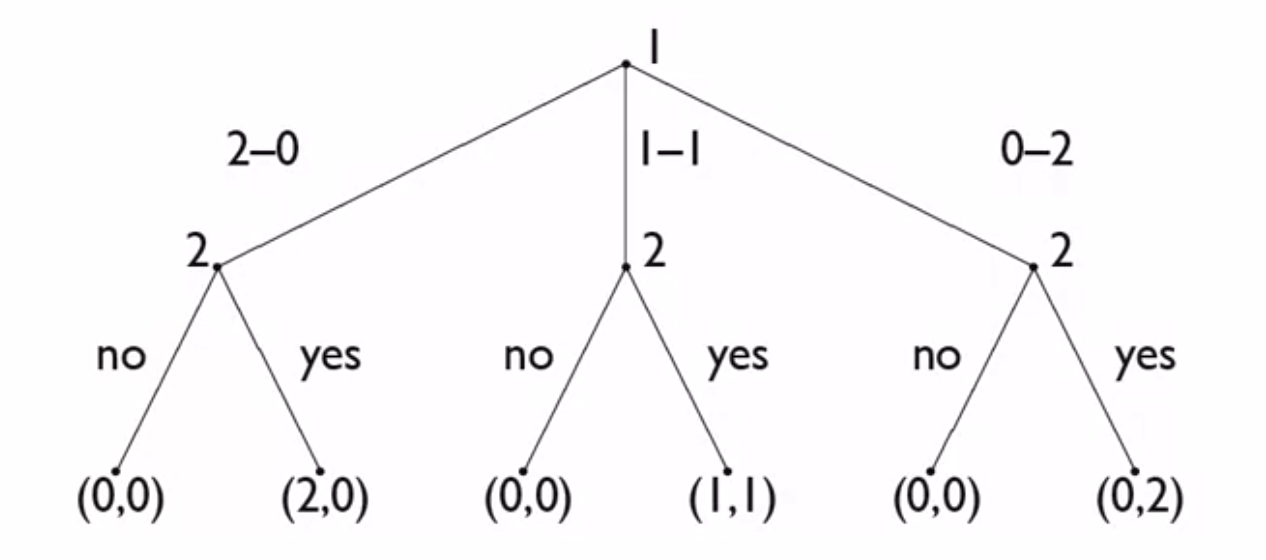
\includegraphics[scale=0.5]{sharetree}
\end{center}
Consider the pure strategies available to player 1 and 2.
\begin{itemize}
\item Player 1 can play a total of 3 pure strategies in the game
\item Player 2 has to choose between yes and no at each node. The action must belong to the set $S= \{ (a,b,c): a,b,c \in \{yes, no\}\} $. So, there are a total of $2^3 = 8$ pure strategies for the player.
\end{itemize}

The definitions of \textbf{mixed-strategy, best response} and \textbf{Nash Equilibrium} are exactly the same here.
\begin{flushleft}
\textbf{Induced Normal Form Game}
\end{flushleft}
We can transform a perfect-information game into a normal form game (as we have complete information and all the possible strategies).

In the following example, we transform a perfect-information game into normal form. The strategy profiles for corresponding players being $$S_1 =\{(A,G), (A,H), (B,G), (B,H)\} $$ $$S_2=\{ (C,E), (C,F), (D,E), (D,F)\}$$
\begin{center}
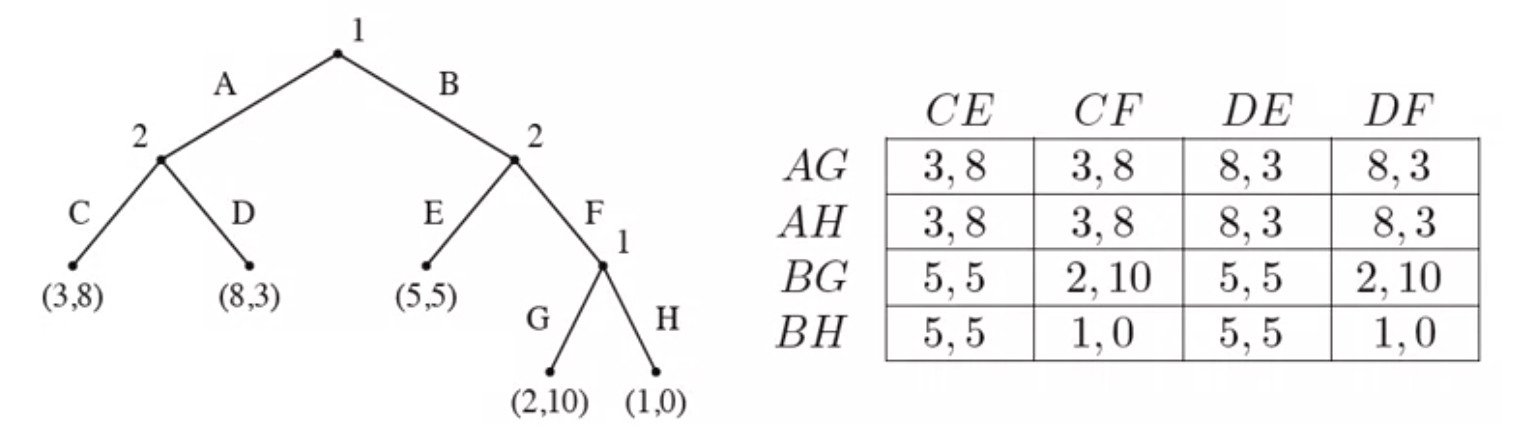
\includegraphics[scale=0.5]{normal}
\end{center}
Pure strategy Equilibria in the above example are:-\\
(A,G),(C,F)\\
(A,H),(C,F)\\
(B,H),(C,E)\\

\subsubsection{Subgame Perfection}

\textbf{Subgame}\\
The \textit{subgame of $G$ rooted at $h$} is the restriction of $G$ to the descendants of $H$.\\
\textbf{Subgames of G}\\
The \textit{set of subgames of $G$} is defined by the subgames of $G$ rooted at each of the nodes in $G$.

\begin{flushleft}
\textbf{Definition}
\end{flushleft}
$s$ is a \textit{subgame perfect equilibrium} of $G$ iff for any subgame $G'$ of $G$, the restriction of $s$ to $G'$ is a Nash Equilibrium of $G'$\\

Note:
\begin{itemize}
\item SInce $G$ is its own subgame, every \textit{subgame perfect equilibrium} is a \textit{Nash Equilibrium}
\item this definition rules out non-credible threats
\end{itemize}

\subsubsection{Backward Induction}

Backward induction in a perfect-information is an iterative process of reasoning backward in time, from the end of a problem or situation, to solve finite extensive form games, and infer a sequence of optimal actions.\\

At each stage of the game it determines the optimal strategy of the player who makes the last move in the game. Then, the optimal action of the next-to-last moving player is determined, taking the last player's action as given. This process continues backward until the best action for every point in time has been determined. Effectively, one is determining the Nash equilibrium of each subgame of the original game.

\subsection{Imperfect Information Extensive Form Games}

Unlike perfect-information games, here, an agent won't have the knowledge of the opponent's moves at every single choice node and cannot plan a best response accordingly. Rather here, players consider some choice nodes to be equivalent to each other and they won't be able to tell them apart. This can be achieved by taking all the sets of equivalent choice nodes and putting them in \textit{equivalence classes}. \\
Now, the player won't have an idea about his exact position in the tree, but knows he was at some choice node belonging to the class where he took the action with the property that each choice node in a class has the same set of actions.
\begin{flushleft}
\textbf{Definition}
\end{flushleft}
In formal terms, An \textit{imperfect-information game} (in extensive form) is a tuple $(N, A, H, Z, \chi,  \rho, \sigma, u, I)$, where
\begin{itemize}
\item $(N, A, H, Z, \chi,  \rho, \sigma, u)$ is a perfect-information extensive-form game, and
\item $I = (I_1, \dots , I_n)$, where $I_i = (I_{i,1}, \dots , I_{i, k_i})$ is an equivalence relation on $\{ h \in H, \rho(h) = i\}$ with the property that $\chi(h) = \chi(h')$ and $\rho(h) = \rho(h')$ whenever there exists a $j$ for which $h \in I_{i,j}$ and $h' \in I_{i,j}$
\end{itemize}

\subsubsection{Strategies}
\begin{flushleft}
\textbf{Pure Strategies}
\end{flushleft}
The pure strategies of player $i$ consists of the cross product $$\prod_{i, j\in I_i} \chi(I_{i,j}) $$ 
Conisder the following example game.
\begin{center}
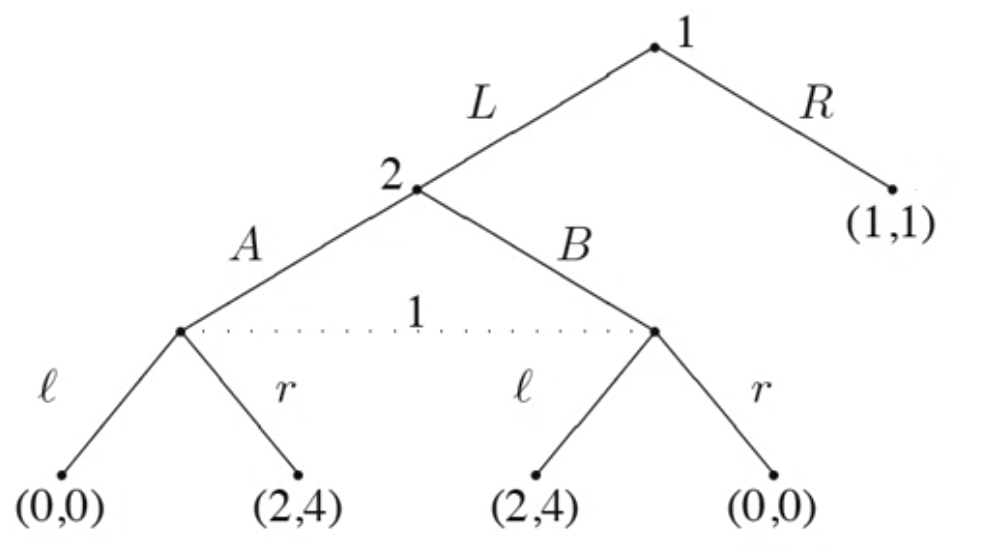
\includegraphics[scale=0.5]{imperfect}
\end{center}
\begin{itemize}
\item If Player 1 goes right, then the  game ends and the payoff is $(1,1)$
\item If Player 1 goes left, Player 2 gets to make a choice between $A$ and $B$, which is unknown to Player 1 and hence the choice nodes for Player 1 are in an equivalence class. Without knowledge of his position, Player 1 has to now move left or right.
\item Nodes of same equivalence class are marked by dotted line as above.
\item Set of pure strategies for Player 1 will be $S_1 =\{(L, l), (L, r), (R, l), (R, r)\}$ and for Player 2 will be $S_2 = \{A, B\}$
\end{itemize}

\subsubsection{Normal-Form Games}
We can represent normal form games in the tree format of imperfect-information game. Consider the \textbf{Prisoners' Dilemma Game} in section 4.3. The game can be represented as a tree in the following manner-
 \begin{center}
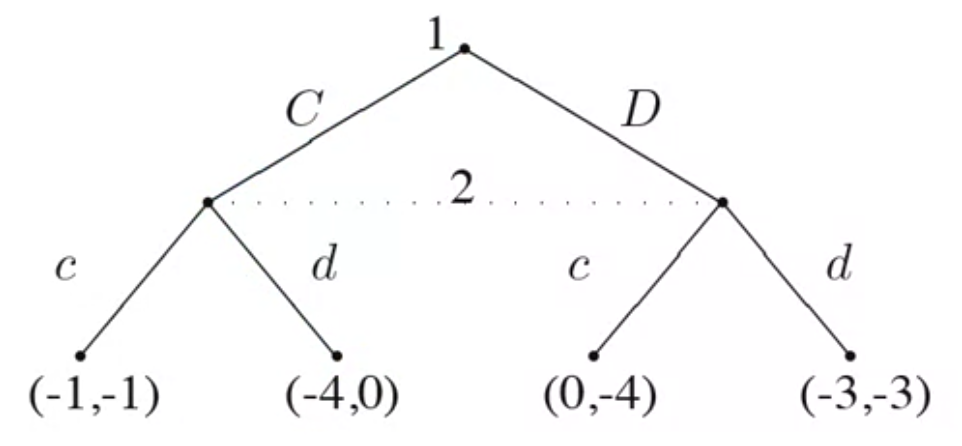
\includegraphics[scale=0.5]{norm}
\end{center}
\begin{itemize}
\item Notice that the order doesn't matter as to who is at the root node because time isn't playing a role in this game
\item The other player has no idea about the first player's moves, hence he has an equivalence class to choose from.
\end{itemize} 
\subsubsection{Mixed and Behavioural Strategies}
There are two meaningfully different kinds of randomized strategies in imperfect-information extensive form games-
\begin{itemize}
\item \textbf{Mixed strategies}-  assign a probability distribution over pure strategies
\item \textbf{Behavioural strategies}- assign, independently for each information set, a probability distribution over actions
\end{itemize}
\pagebreak
\section{Repeated Games}
Till now, the games or situations that were being considered were on a one-time basis, ie. the players faced each other once and moved on. But what happens in real life is there is constant day-to day interactions between the players and that adds up to more than just a single matchup. Hence, we need to repeat the situations and understand the changes that occur in the actions available as well as undertaken by them.

\subsection{Infinitely Repeated Games: Utitlity}
In this, we have a normal form game, and the players play that game over and over again. That means that each player gets a sequence of payoffs that is infinite, and hence cannot use the utility theory to understand it. We can't write it in extensive form as there will be no leaf node for the infinitely deep payoff. Also, we cannot sum up the sequence of payoffs and define utility to be the sum,  because it would be unbounded, and we want a finite one. Instead, we can use the following definition:-\\
\newline
Given an infinite sequence of payoffs $r_1, r_2, \dots$ for player $i$, the \textbf{average reward} for $i$ is $$\lim_{x\to \infty} \sum_{j=1}^{k} \frac{r_j}{k}$$
But technically, this method isn't quite well defined. For example, a player receives a negative payoff early on for a long time,  maybe $100,000$ iterations and positive for the rest, which would result in a positive average reward overall, but hides the fact that the negative payoff early on might be a deal breaker. Hence, we define the term \textbf{discounted reward} as follows:-\\
\newline
Given an infinite sequence of payoffs $r_1, r_2, \dots$ for player $i$ and the discount factor $\beta$ with $0 < \beta < 1$, $i$'s \textbf{future discounted reward} is $$\sum_{j=1}^\infty \beta^j r_j$$
Here the discount factor talks about the value of payoffs for different times.\\
\newline
Two equivalent interpretations of discount factor:
\begin{enumerate}
\item The agent cares more about his well-being in the near term than in the long term
\item The agent cares about the future as much as the present , but with probability $1-\beta$ the game will end in any given round
\end{enumerate}

\subsection{Stochastic Games}
\textbf{Formal Definition:}\\
\newline
A \textbf{stochastic game} is a tuple $(Q, N, A, P, R)$ where-
 
\begin{itemize}
\item $Q$ is a finite set of states
\item $N$ is a finite set of $n$ players
\item $A = A_1 \times \dots \times A_n$ where $A_i$ is a finite set of actions available to player $i$
\item $P: Q \times A \times Q\to [0,1]$ is the transition probability function; $P(q, a, \hat q)$ is the probability of transitioning from state $q$ to $\hat q$ after joint action $a$
\item $R = r_1, \dots, r_n$ where $r_i:  Q \times A \to \mathbb{R}$ is a real valued payoff function for player $i$
\end{itemize}
A stochastic game is a generalization of repeated games where-
\begin{itemize}
\item agents repeatedly play games from a set of normal form games
\item the game played at any iteration depends on the previous game played and on the actions taken by all agents in that game
\end{itemize}
 \begin{center}
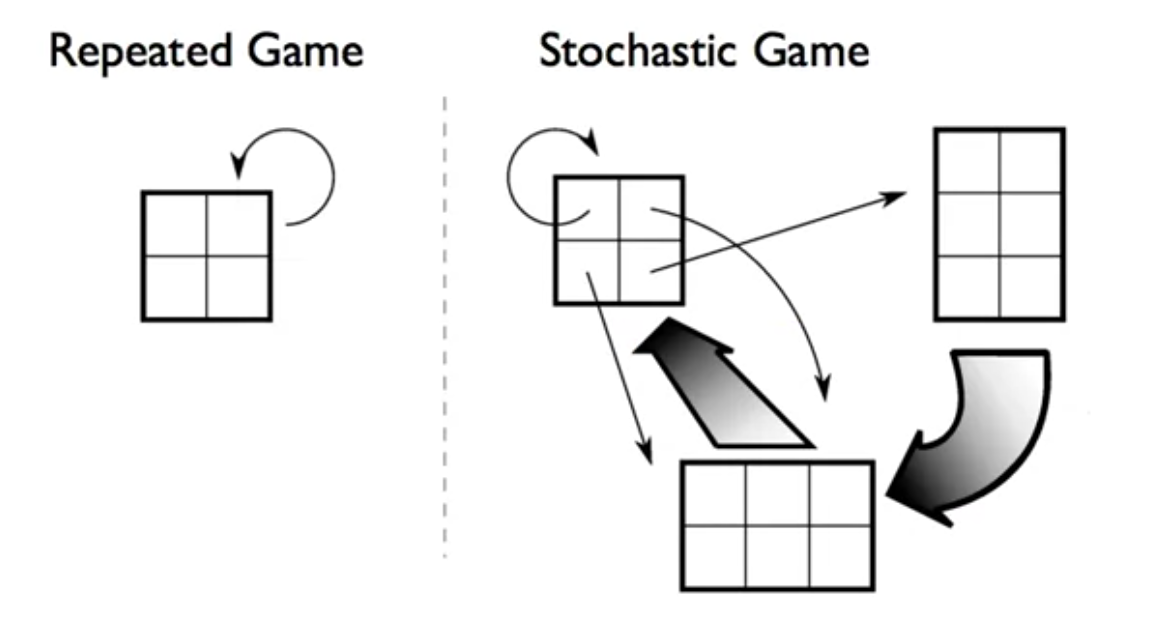
\includegraphics[scale=0.5]{stochastic}\\
An informal visualisation of the  difference between repeated and stochastic games
\end{center}
\subsection{Infinitely Repeated Games: Equilibria}
In an infinitely repeated game your strategy is going to be a choice of action at every decision point that you would have, which means an action that you would take every stage game. And when you take those actions, you actually get to reason about everything that you've seen before in the game ,that is, you can remember all of your own previous actions and you can also remember all of the actions in previous stage games by other players.\\
\newline
So, your pure strategy space is mapping from every history to an action choice that you would make. Clearly, this is an infinite number of actions. So, unlike the previous games we've looked at, extensive form games and normal form games, you're not even going to have a finite set of pure strategies in an infinitely-repeated game.

Some famous pure strategies in such case for Prisoners' Dilemma can be:-
\begin{itemize}
\item \textbf{Tit-for-tat}: Start out cooperating. If the opponent defected, defect in the next round. Then go back to cooperation
\item \textbf{Trigger}: Start out cooperating. If the opponent ever defects, then defect forever
\end{itemize}

\textbf{Some Notations:}\\

Consider any $n$-player game $G = (N, A, u)$ and any payoff vector $r = r_1, r_2, \dots , r_n$\newline
Let $v_i = min_{s_{-i}\in S_{-i}} max_{s_i \in S_i} u_i(s_{-i}, s_i)$\\
$i$'s minimax value: the amount of utility $i$. can get when $-i $ play a minimax strategy against him\\

\textbf{Defintion}:
\begin{itemize}
\item A payoff profile $r$ is \textit{enforceable} if $r_i \geq v_i$
\item A payoff profile $r$ is \textit{feasible} if there exists rational, non-negative values $\alpha_a$ such that for all $i$, we can express $r_i$ as $\sum_{a\in A} \alpha_a u_i(a) $ with $\sum_{a\in A} \alpha_a = 1$
\end{itemize}

\subsubsection{Folk Theorem}

Consider any $n$-player game $G$ and any payoff vector $(r_1, r_2, \dots, r_n)$.
\begin{itemize}
\item If $r$ is the payoff in any Nash equilbrium of the infinitely repeated $G$ with average rewards, then for each player $i$, $r_i$ is enforceable
\item If $r$ is both feasible and enforceable, then $r$ is the payoff in some Nash Equilibrium of the infinitely repeated $G$ with average rewards
\end{itemize}

\subsection{Discounted Repeated Games}
\textbf{Notations:}
\begin{itemize}
\item \textbf{Stage game}: $(N, A, u)$
\item \textbf{Discount Factors}: $\beta_1, \dots, \beta_n, \beta_i \in [0,1]$
\item \textbf{Assume a common discount factor} $\beta_i = \beta$ for all $i$
\item \textbf{Payoff from a play of actions} $a^1, \dots , a^t, \dots:$ $$\sum_t \beta_i^t u_i(a^t)$$
\end{itemize}
\textbf{Histories:}
\begin{itemize}
\item \textbf{Histories of length }$t$: $H^t = \{h_t : h^t = (a_1, \dots, a_t) \in A^t\}$
\item \textbf{All finite histories}: $H = \cup_t H^t$
\item \textbf{A strategy:} $s_i: H \to \Delta(A_i)$ 
\end{itemize}

\subsubsection{Repeated Prisoners' Dilemma}
\begin{itemize}
\item Cooperate as long as everyone has in the past
\item Both players defect forever after if everyone ever deviates: \textit{Grim Trigger}
\end{itemize}
Consider the following matrix:
\begin{center}\begin{tabular}{|c|c|c|} \hline
1/2 & $C$ & $D$ \\ \hline
$C$ & 3,3 & 0,5 \\ \hline
$D$ & 5,0 & 1,1 \\ \hline 
\end{tabular}\end{center}
\begin{itemize}
\item Cooperate from start: $3 + \beta \times 3 + \beta^2 \times 3 + \beta^3 \times 3 \dots = \frac{3}{1-\beta}$
\item Defect from start: $5 + \beta \times 1 + \beta^2 \times 1 + \beta^3 \times 1 \dots = 5 + \beta \times \frac{1}{1-\beta}$
\item Difference : $\beta \times \frac{2}{1-\beta} - 2$
\end{itemize}
The difference is non-negative if $\beta \geq \frac{1}{2}$. So, as long as people care about tomorrow, atleast half as much as today, they're going to be willing to cooperate in this.

But if we increase the incentive to defect from $5$ to $10$, the difference becomes $\beta \frac{2}{1-\beta} -  7$. Which means $\beta \geq \frac{7}{9}$ for the difference to be non-negative, which justifies the intuition that the agent has more urge to defect now than before. 
\subsubsection{Folk Theorem for Discounted Repeated Games}
Consider a finite normal form game $G = (N, A, u)$. Let $a = (a_1, \dots , a_n) $ be a Nash equilibrium of the stage game $G$.\\

If $a'= (a'_1, \dots, a'_n)$ is such that $u_i(a') > u_i(a)$ for all $i$, then there exists a discount factor $\beta < 1$, such that if $\beta_i \geq \beta$ for all $i$, then there exists a subgame perfect equilibrium of the infinite repetition of $G$ that has $a'$ played in every period on the equilibrium path
\pagebreak
\section{Bayesian Games}

\subsection{First Definition}
A set of games that differ only in their payoffs, a common prior defined over them, and a partition structure over the game for each agent.\\

\textbf{Formally speaking:}

A \textit{Bayesian game} is a tuple $(N, G, P, I)$ where
\begin{itemize}
\item $N$ is a set of agents
\item $G$ is a set of games with $N$ agents each such that if $g, g' \in G$ then for each agent $i \in N$ the strategy space in $g$ is identical to the strategy space in $g'$
\item $P \in \prod(G)$ is a common prior over games, where $\prod(G) $ is the set of all probability distributions over $G$
\item $I = (I_1, \dots , I_N) $ is a set of partitions of $G$, one for each agent
\end{itemize}

Example:\\
 \begin{center}
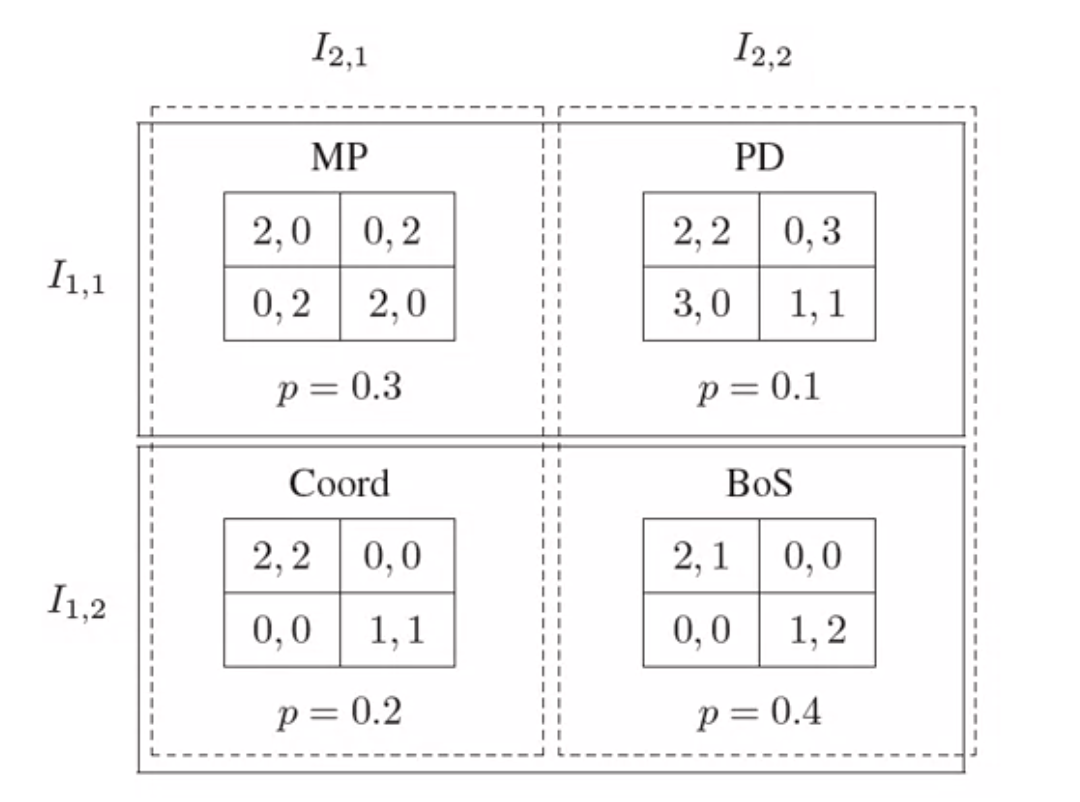
\includegraphics[scale=0.4]{bayesian}\\
\begin{flushleft}
Key:\\
MP - Matching Pennies\\
PD - Prisoners' Dilemma\\
Coord - Coordination Game\\
BoS - Battle of the Sexes
\end{flushleft}
\end{center}
It is going to be randomly decided which game is to be played by the probability factor provided for each game.\\
Here, player 1 won't be able to distinguish between the two games in the first row as well as the two games in the second row. Similar case stands for player 2 with respect to the columns. What this means is that when the players are deciding what action to take, they're going to have to play an action without fully knowing what game is going to be played. And they're going to have to reason about what their opponent is doing without fully knowing what the opponent is going to think. They know the common prior, they know their own equivalence classes and they also know their opponent's equivalence classes.

\subsection{Second Definition}

Directly represent uncertainty over utility function using the notion of \textbf{epistemic types}.\\
Definition:\\
 A  \textit{Bayesian game} is a tuple $(N, A, \Theta, p, u)$ where
\begin{itemize}
\item $N$ is a set of agents
\item $A = (A_1, \dots, A_n)$, where $A_i$ is a set of actions available to player $i$
\item $\Theta = (\Theta_1, \dots , \Theta_n)$ where $\Theta_i$ is the type space of player $i$
\item $p: \Theta \to [0,1] $ is the common prior over types
\item $u = (u_1, \dots, u_n)$,  where $u_i: A \times \Theta \to \mathbb{R}$ is the utility function for player $i$
\end{itemize}
 \begin{center}
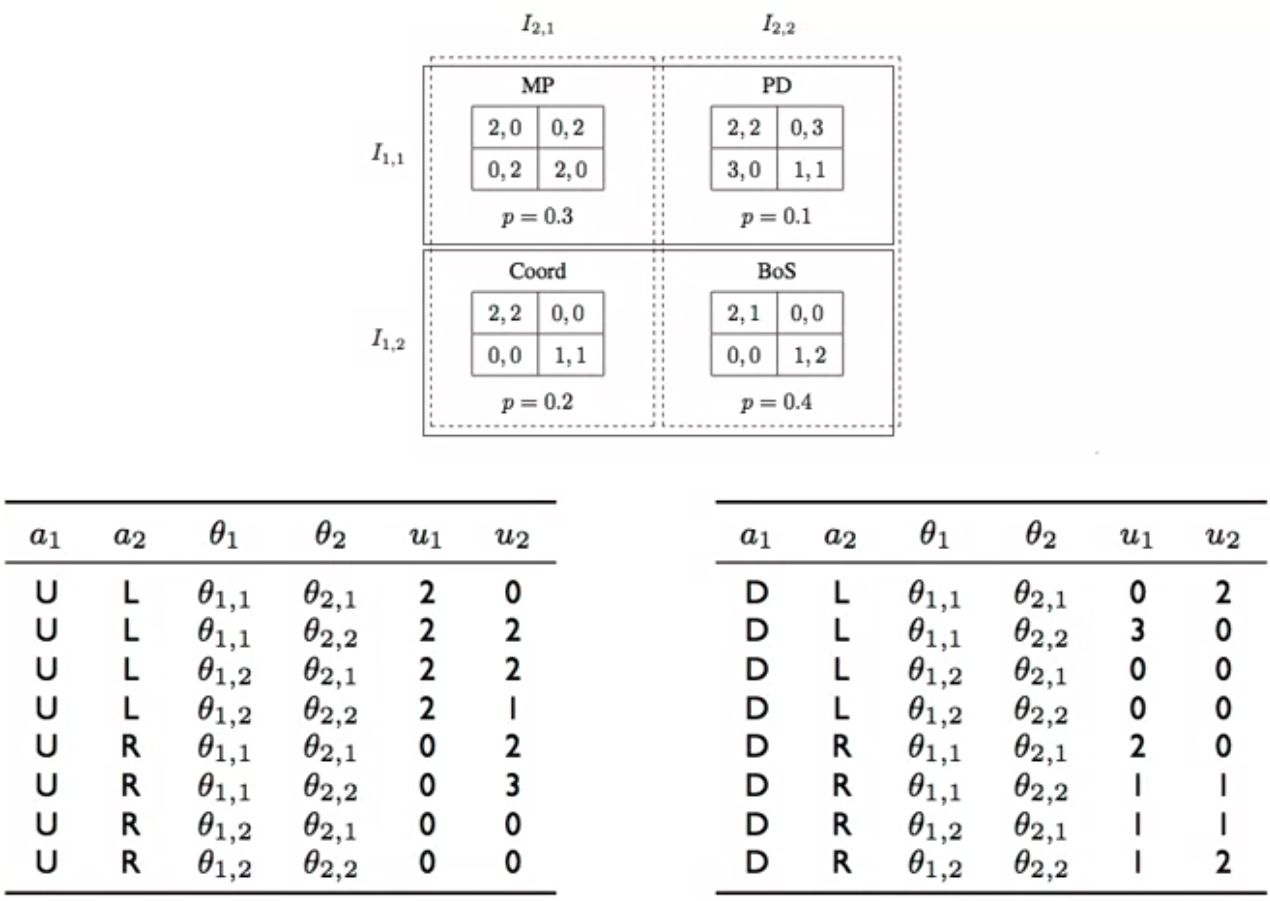
\includegraphics[scale=0.4]{bayesian2}\\
In this figure all the possible moves have been listed out for player 1 and 2, with their corresponding utilities
\end{center}

\subsection{Analyzing Bayesian games}
\subsubsection{Strategies}
Given a Bayesian game $(N, A, \Theta, p, u)$ with finite set of players, actions and types, strategies are defined as follows:
\begin{itemize}
\item \textbf{Pure strategy}: $s_i: \Theta_i \to A_i$
	\begin{itemize}
	\item a choice of a pure action of player $i$ as a function of his or her type
	\end{itemize}
\item \textbf{Mixed strategy}: $s_i: \Theta_i \to \prod(A_i)$
	\begin{itemize}
	\item a choice of a mixed action of player $i$ as a function of his or her type
	\end{itemize}
\end{itemize}
\subsubsection{Expected Utility}
Three standard notions of expected utility are defined.
\begin{itemize}
\item \textit{ex-ante}: The agent knows nothing about anyone's actual type
\item \textit{interim}: an agent knows her own type but not the types of the other agents
\item \textit{ex-post}: the agent knows all agents' types
\end{itemize}
\textbf{Interim Expected Utility}:\\
\begin{itemize}
\item Given a Bayesian game $(N, A, \Theta, p, u)$ with finite set of players, actions and types, $i$'s \textit{interim expected utility} with respect to type $\theta_i$ and a mixed strategy profile $s$ is $$EU_i(s|\theta_i) = \sum_{\theta_{-i} \in \Theta_{-i}}p(\theta_{-i}| \theta_i) \sum_{a \in A}(\prod_{j\in N}s_j(a_j|\theta_j))u_i(a, \theta_i, \theta_{-i})$$
\item $i$'s \textit{ex ante expected utility} with respect to a mixed strategy profile $s$ is $$EU_i(s) = \sum_{\theta_i \in \Theta_I}p(\theta_i)EU_i(s|\theta_i)$$
\end{itemize}
\subsubsection{Bayesian (Nash) Equilibrium}
A Bayesian equilibrium is a mized strategy profile $s$ that satisfies $$s_i \in argmax_{s'_i}EU_i(s'_i,s_{-i}|\theta_i)$$ for each $i$ and $\theta_i \in \Theta_i$\\
If $p(\theta_i)>0$ for all $\theta_i \in \Theta_I$, then this is equivalent to requiring that $$s_i \in argmax_{s'_i}EU_i(s'_i,s_{-i}|\theta_i) = argmax_{s'_i} \sum_{\theta_i}EU_i(s'_i, s_{-i}|\theta_i)$$ for each $i$
\subsection{A Sheriff's Dilemma (Example)}
A sheriff faces an armed suspect and they must simultaneously decide whether to shoot or not :
\begin{itemize}
\item the suspect is a criminal with probability $p$
\item the sheriff would rather shoot if the suspect shoots, but not if the suspect does not
\item the criminal would rather shoot even if the sheriff does not , as the criminal would be caught if does no shooting
\item the innocent suspect would  rather not shoot even if the sheriff shoots
\end{itemize}
Payoff Structure:
\begin{center}\begin{tabular}{|c|c|c|} \hline
Good & $Shoot$ & $Not$ \\ \hline
$Shoot$ & -3,-1 & -1,-2 \\ \hline
$Not$ & -2,-1 & 0,0 \\ \hline 
\end{tabular}\hspace{1.0cm}\begin{tabular}{|c|c|c|} \hline
Bad & $Shoot$ & $Not$ \\ \hline
$Shoot$ & 0,0 & 2,-2 \\ \hline
$Not$ & -2,-1 & -1,1 \\ \hline 
\end{tabular}\end{center}
Upon analysis, if the suspect is good, it is strategically strictly dominant not to shoot. If the suspect is bad, then from the second matrix, it would be a strictly dominant strategy to shoot. \\
So, if the suspect is bad with a probability $p$ and good with probability $1-p$, then the sheriff's best reply would be- 
\begin{itemize}
\item If he chooses to shoot, the payoff would be $-1(1-p) + 0(p)$
\item if he chooses not to, then payoff would be $0(1-p) + 2(p)$
\item Hence, on equating, we see that when $p > 1/3$ the sheriff would have a better incentive to shoot, and not otherwise
\end{itemize}
\pagebreak
\section{Coalitional Games}
In game theory, a coalitional game is a game with competition between groups of players ("coalitions") due to the possibility of external enforcement of cooperative behavior. These are opposed to non-cooperative games in which there is either no possibility to forge alliances or all agreements need to be self-enforcing through credible threats\\

Transferable Utility Assumption:
\begin{itemize}
\item payoffs may be redistributed among a coalition's members
\item satisfied whenever payoffs are disposed in a universal currency
\item each coalition can be assigned a single value as its payoff
\end{itemize}

\subsection{Coalitional Game with Transferable Utility}
A \textit{coalitional game with transferable utility} is a pair $(N, v)$, where 
\begin{itemize}
\item $N$ is a finite set of players indexed by $i$
\item $v : 2^N \to \mathbb{R}$ associates with each coalition $S \subseteq N$ a real-valued payoff $v(S)$ that the coalition's members can distribute among themselves, assuming $v(i\ne 0) = 0$ 
\end{itemize}

This type of game theory helps us to answer which coalition is more likely to form and how should the coalition divide its payoff among its members

\subsection{Superadditive Games}
A game $G = (N, v)$ is \textit{superadditive} if for all $S, T\subset N$, if $S \cap T \ne 0$ , then $v(S\cup T)\geq v(S) + v(T)$\\
\newline
It is justified when coalitions can always work without interfering with one another.\\ The value of two coalitions will be no less than the sum of their individual values, which implies grand coalition has the highest payoff.\\
We need to define the 'fair' way for a coalition to divide its payoff. To do this, we can identify axioms that express properties of a fair payoff division.

\subsection{The Shapley Value and Axioms}
\textit{Lloyd Shapley's} Idea: Members should receive payoffs or shares proportional to their marginal contributions.\\
But this can be tricky to fix. Let's take an example. Suppose that everybody together in a society can generate 1, but if we're
missing any member of society we get 0. Hence, we can write:\\
\begin{itemize}
\item $v(N) = 1, v(S)=0$ if $N\ne S$
\item Then $v(N) - v(n/\{i\}) = 1$ for every $i$, everybody's marginal contribution is 1, everybody is essential to generating any value, but we cannot pay everybody equally.
\end{itemize}
\subsubsection{Shapley's Axioms}
\begin{enumerate}
\item \textbf{Symmetry}: For any $v$, if $i$ and $j$ are interchangeable, then $\psi_i(N, v) = \psi_j(N, v)$
\item \textbf{Dummy Player}: For any $v$, if $i$ is a dummy player then $\psi_i(N, v)=0$
\item \textbf{Additivity}: For any two $v_1$ and $v_2$, $\psi_i(N, v_1 + v_2) =\psi_i(N, v_1) + \psi_i(N, v_2)$ for each $i$, where the game $(N, v_1+v_2)$ is defined by $(v_1 + v_2)(S) = v_1(S) + v_2(S)$ for every coalition $S$
\end{enumerate}
\subsubsection{Shapley Value}
Given a coalition $(N, v)$, the \textit{Shapley Value} divides payoffs among players according to:
$$\phi_i(N, v) = \frac{1}{N!}\sum_{S \subseteq N / \{i\}} |S|!(|N| - |S| - 1)! [v(S\cup \{i\})- v(S)]$$ for each player $i$\\
\textbf{Theorem}:\\

Given a coalitional game $(N, v)$, there is a unique payoff division $x(v) = \phi(N, v)$ that divides the full payoff of grand coalition and that satisfies the \textit{Symmetry, Dummy player} and \textit{Additivity} axioms: the Shapley Value

\subsection{The Core}
Core is an alternative coalitional game theory concept to the Shapley Value. Shapley value told us about how to divide the coalition's value fairly among all of its members. Instead we have to consider whether the agents would be willing to form the grand coalition, as compared to forming smaller coalitions that might give all of their members greater value than they're able to achieve in the grand coalition.
\subsubsection{The Voting Game: Example}
A parliament is made up of four political parties, A, B, C and D, which have 45, 25, 15 and 15 representatives respectively. They are to vote on whether to pass a \$100 million spending bill and hoe much of this amount should be controlled by each of the parties. A majority vote, a minimum of 51, is required to pass any legislation, and if bill does not pass then every party gets nothing to spend.\\                                                                                                                                                                 
Corresponding Shapley Value: $(50, 16.67, 16.67, 16.67)$\\        
\newline                                                                      
This leads to a thought if a sub-coalition can gain from it more. While A can't obtain more than 50 on its own, A and B have incentive to defect and divide 100 million between them.\\
Under what conditions would the agents want to form a grand coalition. They would want to do so if and only if the payment profile is drawn from a set called the core.
\subsubsection{Core: Definition}
A payoff vector $x$ is in the core of a coalitional game $(N, v)$ iff $$\forall S \subseteq N, \sum_{i\in S} x_i \geq v(S)$$
\textbf{Existence and Uniqueness}:\\
Core need not be present always, ie. it can be empty, and the core is not unique, there can exist more than one type of distribution\\
\textbf{Simple Game}: A game $G$ is \textit{simple} if for all $S \subset N, v(S) \in \{0, 1\}$\\
\textbf{Veto Player}: A player $i$ is a \textit{veto player} if $v(N/ \{i\}) = 0$\\
\newline
\textbf{Theorem:}\\
In a simple game the core is empty iff there is no veto player. If there are veto players, then the core consists of all payoff vectors in which the non-veto players receive 0.

\subsubsection{Airport Game: Example}
Several nearby cities need airport capacity, with different cities needing to accommodate aircrafts of different sizes. If a new regional airport is built the cities will have to share its cost, which will depend on the largest aircraft the runway can accommodate. Otherwise each city will have to build its own airport.\\
This situation can be modeled as a coalitional game $(N, v)$, where $N$ is the set of cities, and $v(S)$ is the sum of costs of building runways for each city in $S$ minus the cost of the largest runway required by any city in $S$.\\
\newline
\textbf{Convex Game}: A game $G$ is \textit{convex} if for all $S, T \subset N,$  $ v(S\cup N) \geq v(S)+ v(T) - v(S \cap T)$
\begin{itemize}
\item Every convex game has a non-empty core
\item In every convex game, the Shapley value is in the core
\end{itemize}
\end{document}  